\documentclass{beamer}
\usepackage{graphicx}
\usetheme{Boadilla}
\newcommand{\ba}{\overline}
\definecolor{resulthead}{RGB}{205,205,235}
\definecolor{termshead}{RGB}{242,218,195}
\begin{document}

\title[Math and Proofs]{Math and Proofs Class 4}
\date{October 17th, 2017}

\begin{frame}[plain]
\titlepage
\end{frame}

\begin{frame}{Fun aside: Chomp Game}
\begin{figure}
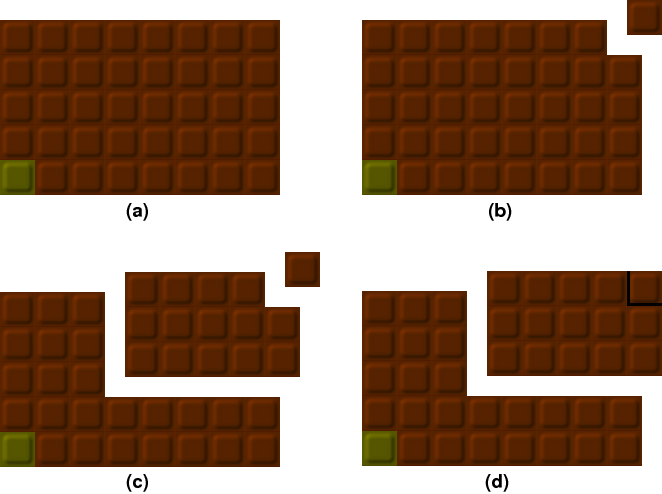
\includegraphics[scale=0.5]{Chomp.png}
\caption{Chomp}
\end{figure}
\end{frame}

\begin{frame}{Recap of Last Class}
\begin{itemize}
\item We did some more set theory!
\item Now we'll use set theory and look at equivalence relations, functions, and bijections
\end{itemize}
\end{frame}

\begin{frame}{Equivalence Relations}
\begin{itemize}
\item An \emph{equivalence relation} on a set $A$ is a set of ordered pairs where each half of each pair is an element of $A$
\item It also has to be these three things:
\begin{enumerate}
\item Reflexive: $(a,a)$ is in the equivalence relation for every $a\in A$.
\item Symmetric: If $(a,b)$ is in the equivalence relation, then so is $(b,a)$.
\item Transitive: If $(a,b)$ and $(b,c)$ are in the equivalence relation, then so is $(a,c)$.
\end{enumerate}
\item Let $A = \{1,2,3\}$. We're going to see what is and isn't an equivalence relation on $A$.
\end{itemize}
\end{frame}

\begin{frame}{Functions}
\begin{itemize}
\item A \emph{function} $f:A\to B$ is a set of ordered pairs in $A\times B$ so that each element of $A$ appears in exactly one ordered pair.
\item Exercise: Let $A = \{1,2,3\}, B = \{a,b,c\}$. Which of the following sets are functions?
\begin{enumerate}
\item $\{(1,a), (2,b), (3,c)\}$
\item $\{(1,b), (2,b), (3,b)\}$
\item $\{(1,a), (1,b), (3,c)\}$
\item $\{(2,c), (1,b), (3,a)\}$
\end{enumerate}
\item What you might think of as a ``normal function'' is also a function by this definition
\begin{itemize}
\item The function $y = x^2$ corresponds to the set $\{(x,x^2): x\in\mathbb{R}\}$, which is the set of all pairs of numbers where the first number can be anything but the second number is the first one squared.
\end{itemize}
\end{itemize}
\end{frame}

\begin{frame}{Bijections}
\begin{itemize}
\item A \emph{bijection} is a function where each output appears exactly once too.
\item Exercise: Let $A = \{1,2,3\}, B = \{a,b,c\}$. Which of the following sets are functions?
\begin{enumerate}
\item $\{(1,a), (2,b), (3,c)\}$
\item $\{(1,b), (2,b), (3,b)\}$
\item $\{(1,a), (1,b), (3,c)\}$
\item $\{(2,c), (1,b), (3,a)\}$
\end{enumerate}
\item Since each input has to appear exactly once and each output has to appear exactly once, a bijection is a ``pairing off'' of the first set and the second set
\item So what happens if there are different numbers of elements -- you can't have a bijection!
\end{itemize}
\end{frame}

\begin{frame}{Cardinality}
\begin{itemize}
\item Let's make an equivalence relation between different sets
\item Two sets $A$ and $B$ are equivalent if there's a bijection between them.
\item Remember what this means: $A$ and $B$ are equivalent if they have the same $\mathbf{number}$ of elements
\item Let's check that this actually is an equivalence relation: reflexive, symmetric, transitive
\item We call this concept cardinality
\end{itemize}
\end{frame}

\begin{frame}{Next Time}
\begin{itemize}
\item We'll look at cardinality and infinity
\end{itemize}
\end{frame}

\end{document}